\chapter{Productive Abstractions of Cache Coherence Policies}
\label{c.coherence}

In a multicore chip with a sizeable hierarchy of on-chip caches,
the majority of the data movement activity that occurs within the chip
is done automatically, in accordance with a cache coherence protocol.
The cache coherence protocol is a distributed protocol implemented by a system of cache controllers and memory controllers
spread across the chip that communicate through on-chip networks.
As traditional cache coherence protocols preserve the software abstraction of a global memory shared by all the cores,
the controllers must work behind-the-scenes to keep copies of data in the right places,
while managing tradeoffs between communication volume, storage capacity and performance.
Going forward, due to the increased percentage of energy consumpution taken up by the memory hierarchy,
we predict the rise of customizable, heterogeneous cache coherence policies.
Specifically, protocols that minimize data movement for particular use cases
will become an increasingly desirable feature of an on-chip memory hierarchy.
How to define customizable coherence policies, implement the associated protocols efficiently,
and manage the aforementioned communication/performance tradeoff is an important design challenge for future energy-efficient architectures. 

Unfortunately, designing more complex, customizable cache coherence protocols is not a task hardware engineers can easily take on.
Protocol correctness can be determined via formal analysis of an abstract model of the protocol and memory system.
However, there are a huge number of ways in which details of the concrete implementation can undermine abstract correctness.
As in any distributed system, modules designed by different teams may interact in unexpected ways,
and assumptions about atomically visible behaviors or event priority levels may be violated,
leading to corrupted data or system deadlock.
Hardware designers shoulder the burden of maintaining the implicit semantics of the abstracted protocol model
throughout the concrete controllers and networks that they build.
This chapter proposes that improving the capabilities of hardware description languages (HDLs) offers us a path forward to lighten this design burden.
By raising the level of abstraction at which cache controller logic can be described,
and from which synthesizable designs can be generated,
we can smooth over the gap between protocol specification and implementation.

A coherence protocol specifies the exact sequences of messages that must be propagated through the memory hierarchy in order to service memory operations,
while preserving the Single-Writer-Multiple-Reader invariant throughout a logical epoch.
Preserving this invariant implies that the system creates a global total ordering of reads and write to any given memory location.
Because metadata related to the permissions available on each cache block are distributed throughout the cache hierarchy,
implementing a protocol becomes an exercise in atomically applying metadata updates across a distributed storage system.
This mindset leads us to consider an approach to specifying coherence protocols based on transactions
and factoring out the expression of the transactions from their content and implementation.

In the previous chapter, I presented TileLink,
a protocol framework designed to be a substrate for cache coherence transactions that implement a particular cache coherence policy. 
TileLink provides structure by defining sequences of messages that can be sent between interacting, coherent agents in order
to implement a protocol that is guaranteed to be deadlock free in a nested, hierarchical memory system.
However, TileLink by design says nothing about the particular details of the coherence policy,
which drives the creation and use of these message types.
Filling in details is a task left up to the designers of the cache controllers.

This chapter fills in the aforementioned gaps in the TileLink framework by introducing two further abstractions.
The first is a high-level language,
called \emph{message flows},
taken from the verification literature, 
that describes all the global transactions that make up a particular coherence protocol.
A collection of flows describes every sequence of actions that a protocol can take,
where actions consist of sending TileLink messages and accessing  data and metadata in local memories.
The second abstraction is \emph{coherence metadata objects}.
These objects encapsulate the states that distinguish protocol message flows from one another
and provide methods for generating TileLink messages and making policy-based decisions within flow transactions.
The abstraction provided by the metadata objects separates the concerns of the controller design from the concerns of the policy design, 
while the underlying TileLink substrate ensures forward progress of global protocol transactions.

\section{Background} 

Designing new cache coherence protocols or supporting a wider variety of more complicated protocols is not a task hardware engineers should underestimate.
Verifying the correctness of a cache coherence protocol is a challenging task, and
verifying that a correct protocol has been implemented correctly (using simulations or silicon) is even more difficult
\cite{deorio2008post, bentley2001validating, burckhardt2005verifying, clarke1995verification, dill1992protocol, wood1990verifying}.
Traditionally, protocol correctness is verified using an abstracted version of the distributed system of caches upon which the protocol operates
\cite{talupur2008going, delzanno2003constraint, pong1997verification, wood1990verifying, mcmillan2001parameterized}.
The abstraction employed at this stage makes the verification process tractable by eliding many details of the underlying modules' implementations.
Upon verification of protocol correctness, hardware designers must then use a HDL to write cache controller logic that correctly implements the protocol.
Unfortuntately, the semantic gap between high-level abstract descriptions of protocols and 
concrete HDL implementations of those same protocols is so wide that verifying the correctness of the protocol
does not come close to guaranteeing the correctness of the final implementation \cite{dave-memocode05}.

I am not the first to propose using a higher level of abstraction to describe cache coherence protocol behavior
in such a way that cache controller implementations can be synthetized from the same description that has been verified.
The following approaches each offer a Domain Specific Language (DSL)
built around an abstraction of state machines that perform certain actions when certain conditions are met.
This conditional execution model is a good fit for the requirements of a coherent cache controller,
which must update metadata and data based on a series of messages it sends and receives.
Each high-level description is used to drive the creation of implementations (synthetizable hardware or simulator code),
as well as correctness (verification rules or documentation) from the same source.

Teapot \cite{chandra-dsl97, chandra-sigplan96}
is a Pascal-like DSL for describing coherence protocols using ``continuations'' as an abstraction.
A Teapot program consists of a set of states; each state
specifies a set of message types and the actions to be
taken on receipt of each message, should it arrive for a
cache block in that state.
Teapot provides suspend/resume semantics within each state-based description;
these continuations are used to automatically infer the set of intermediate states and handle unexpected messages.
Continuations in Teapot allow developers to avoid having to manually decompose
a handler into atomically executable pieces and sequence them. 
Teapot outputs C code for distributed memory implementations and $Mur\phi$ models for verification.

Bluespec SystemVerilog (BSV) \cite{bluespec}
is an HDL that produces synthesizeable hardware implementations based on an absraction called \emph{guarded atomic actions} (GAAs).
BSV has been proposed as a particularly suitable language for describing distributed cache coherence controllers \cite{dave-memocode05}.
GAAs consist of a guard (boolean logic predicate) and an action (some kind of state update)
that is executed atomically by the hardware control logic when the predicate evaluates to true.
Becuase GAAs are also an abstraction that are compatible with many formal verification tools,
and because the BSV compiler produces implementations of rules automatically,
verification overhead for implementations of coherence protocols in this language should be reduced.

The gem5 simulation environment \cite{binkert-sigarch11}
provides SLICC, a DSL for generating state machines for coherence protocols.
SLICC consists of descriptions of individual controller state machines in terms of events, as well as the set of available message types
used to communicate between controllers.
The SLICC compiler outputs C++ simulator code and HTML documentation.

All of the above approaches are based on specifying local descriptions of pieces of a global coherence transaction;
when the state machines they describe are interconnected, the intention is to produce correct global behavior.
This approach reflects a bottom-up philosophy to protocol implementation.
In contrast, we wished to adopt a top-down approach, wherein a global description of transactions
is decomposed into local sub-transactions, which then drive the design of the individual controllers.
We therefore turned to the verification literature to find verification strategies based on expressing global descriptions of protocol behavior.

While many transactional models of coherence protocols have been proposed,
the one best suited to our goals was the \emph{message flow} approach to parameterized protocol verification
\cite{talupur2008going, oleary-fmcad09}.
A message flow is a sequence of messages sent among agents following a protocol that
logically constitutes a single transaction of the protocol. 
In the next section, we discuss how a global, flow-based description of a protocol can be decomposed into a set
of local controller transactions, as well as how we implement those local transactions in Chisel,
our meta-HDL embedded in Scala.

So far we have discussed prior art in how to implement protocols,
but we should also review what protocols to consider implementing.
Heterogeneity in memory access behavior as been a major focus of study for distributed shared memory systems.
Memory access patterns can generally be grouped at a high level into a few common sharing patterns, such as read-modify-write, producer-consumer, and migratory.
Systems that support adaptive cache coherence protocols allow the behavior of the protocol to change with detected changes in program behavior.
There are many examples of such adaptive protocols in the distributed memory space,
including \cite{amza-hpca97,lebeck-archnews95,stenstrom-isca93,cox-isca93}.
Note that these designs have a single protocol, but one that varies its behavior dynamically.
In particular, we used two academic proposals~\cite{stenstrom-isca93,cox-isca93} as inspiration for the migratory policy provided in our Rocket Chip Generator~\cite{rocket}.

In the shared memory space, designs like FLASH \cite{kuskin-archnews94} have incorporated multiple protocols on top of a single hardware substrate in order to provide adaptability. Generally, transitions between protocols have been triggered by heuristic mechanisms \cite{mukherjee-archnews98}. Others \cite{chandra-sigplan96,falsafi-sc94} have proposed creating application-specific protocols that are tailored to match a particular application's needs.
These efforts indicate that multiple protocols can share the same underlying communication framework and memory system,
which served as an inspiration for the TileLink/CoherencePolicy separation of interests described in this chapter and the previous.

\section{Protocol Message Flows}

Talupur and Tuttle showed that message flows are a succinct and
readily available source of high-level invariants that have historically gone
unused in the formal verification of cache coherence protocols \cite{talupur2008going}.
Flows are often illustrated by protocol designers in the form of message sequence charts,
which are frequently found in design documents.
Protocol designers use message flows to describe
the basic organization of a protocol and to reason about its requirements.
Message flows impose constraints on the order in which the actions appearing within them can happen:
an action can execute only after any actions it depends upon have been executed.

It is worth noting that the TileLink transactions we illustrated in the previous chapter using message sequence charts
are a form of message flows.
The only information that the flows in that chapter lack is information about what coherence protocol related events take place in between the sending
and receiving of TileLink particular messages.
Thus, TileLink is a framework that describes the shapes of a set of possible flows,
and these outlines can be filled in to create more concrete specifications of protocol behavior.

\begin{figure}
\centering
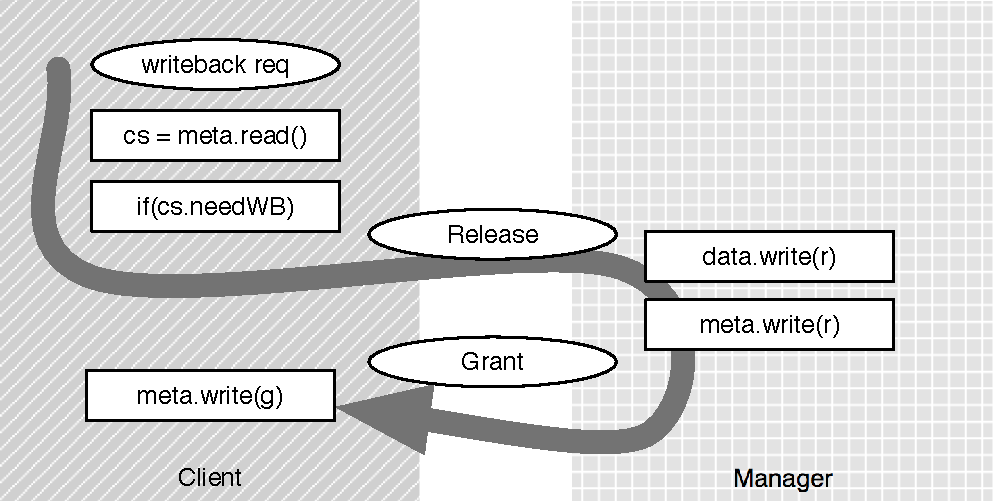
\includegraphics[width=0.8\columnwidth]{coherence/figures/rel-flow.pdf}
\caption[A volunary writeback flow.]{
A voluntary writeback message flow in a single realm.
}
\label{fig:rel-flow}
\end{figure}

\begin{figure}
\centering
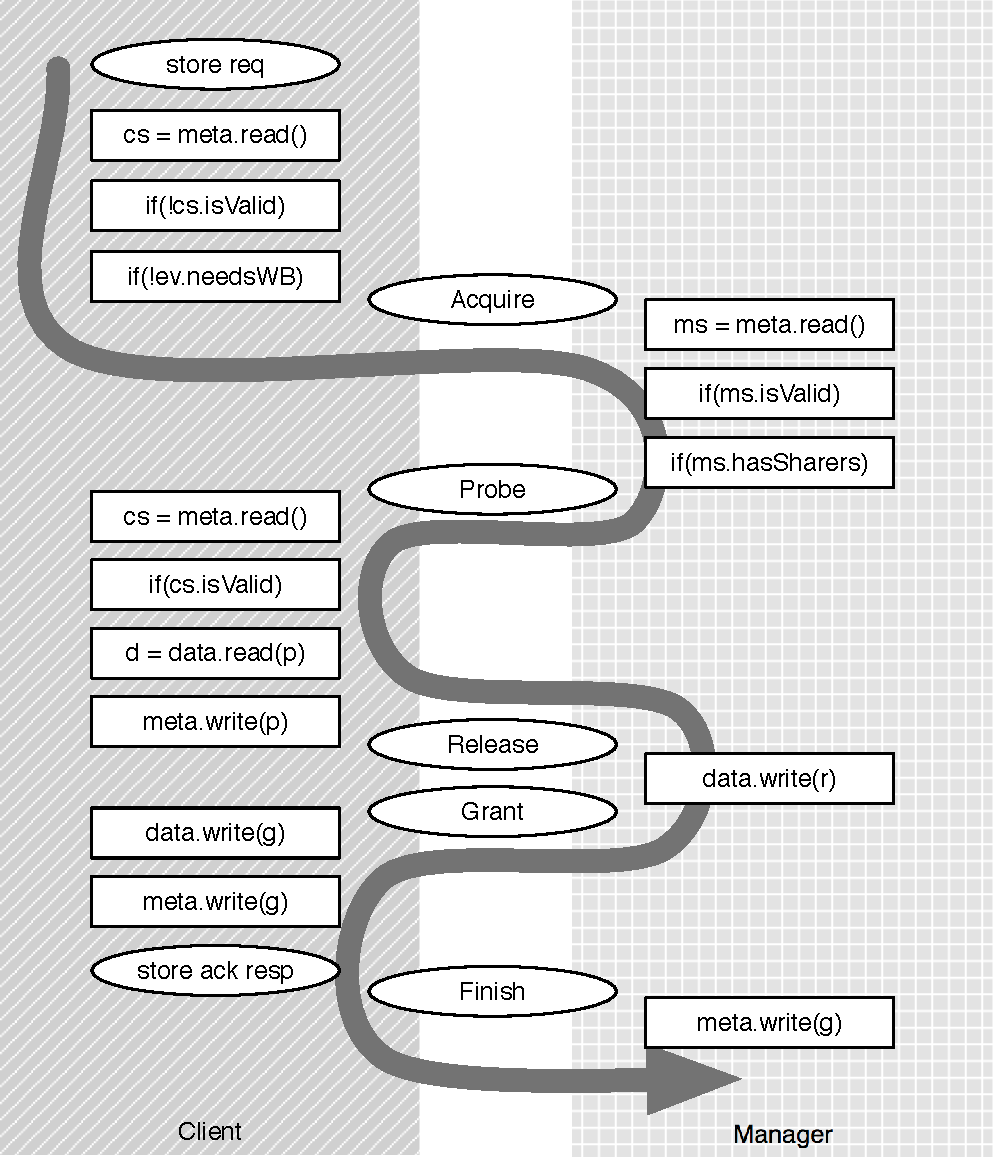
\includegraphics[width=0.8\columnwidth]{coherence/figures/acq-flow.pdf}
\caption[A processor store flow with probes.]{
A processor store flow in a single realm, which must probe other clients in the realm.
}
\label{fig:acq-flow}
\end{figure}

\begin{figure}
\centering
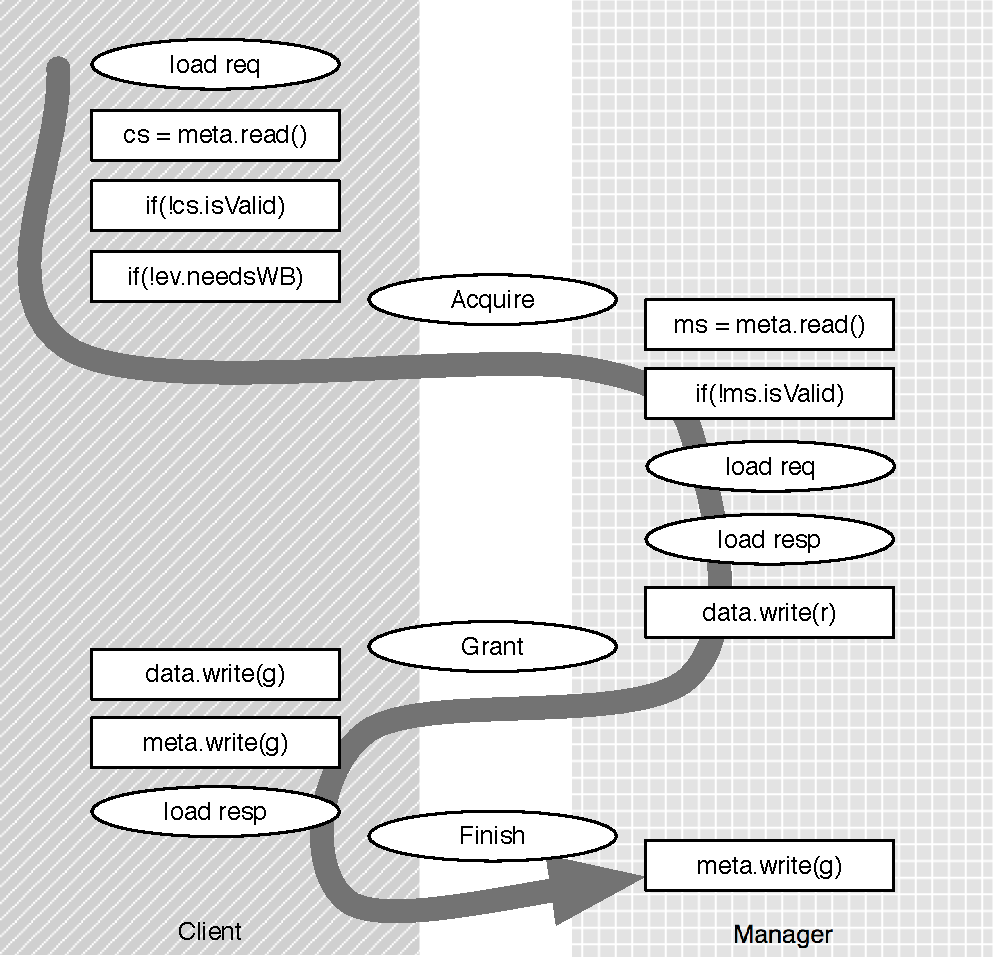
\includegraphics[width=0.8\columnwidth]{coherence/figures/outer-acq-flow.pdf}
\caption[A processor load flow that misses twice.]{
A processor load flow in a single realm, which must make a request to outer memory.
}
\label{fig:outer-acq-flow}
\end{figure}

The simplest flows are linear ordering of events, usually involving two agents.
Each entry in the flow is either a simple event,
corresponding to a single protocol update being committed,
or a \emph{sub-flow} recursively composed of simple events.
Figure~\ref{fig:rel-flow} shows a simple flow based around a voluntary writeback of dirty data from a client cache
using a TileLink Release/Grant transaction.

The notion of sub-flow allows us to
chop up a complicated flow into smaller units such that each
unit shows interaction between two or more agents engaged in a tightly-coupled causal interaction.
An event might have multiple preceding actions,
or might have more than one succeeding event.
Flows may only express a partial order of events and not a total order.
For all of the above reasons, O'Leary et al. proposed that it is best to represent flows as Directed Acyclic Graphs (DAGs)
\cite{oleary-fmcad09}.
Figure~\ref{fig:acq-flow} shows a more complicated flow that involves acquiring write permissions on a block that is currently being
shared by multiple clients, again using a 5-step TileLink transaction.
Figure~\ref{fig:outer-acq-flow} shows annother example flow, one that involves acquiring read permissions on a block that the manager does not possess, forcing it to forward the query to an outer realm.

An important part of verifying protocols using flows is to specify rules that govern non-interference between flows,
i.e., which flows are allowed to execute in the system at the same time.
For our family of coherence protocols, these rules are reflected in the specification of the TileLink substrate
described in the previous chapter.
Correct implementations of TileLink will, by definition, enforce the non-interference rules required by our flows.
While we cannot infer the flow non-interference rules automatically from the TileLink specification,
this congruence is still significant in that it means proofs of a correct TileLink implementation
are sufficient to guarantee correct flow non-interference.

\subsection{From Global Flows to Local Transactions}

Recognizing that a global flow can be divided into sub-flows is useful for providing non-interference lemmas to CMP-based formal verification tools \cite{oleary-fmcad09}.
However, this process also provides a mechanism for us to decompose and re-aggregate the contents of sub-flows based on their geographical location.
In other words, if each flow touches several distinct agents, 
we can collect all those sub-flows applied within an individual type of agent.
Then, if we can generate agent controllers that are capable of performing each sub-flow atomically,
as well as send messages to other agents and wait for responses,
we will have furnished ourselves with a controller that correctly implements the sub-flows of all
possible global flows.
This top-down approach to controller design is central to the productivity of our approach.

In this section, we present an algorithm for turning a collection of flows into multiple collections of localized sub-flows.
First, we express the flows as DAGs in Scala, where vertices are events or actions and edges are happens-before dependencies between them.
Next, we walk each DAG looking for components that are separable sub-graphs of events that all occur at the same agent.
We can sever the graph around these points, leaving us with input vertices that represent receiving a message of a particular type.
These input nodes are the events that kick off local sub-transactions.
Conversely, these mini-DAGs may also contain nodes that require sending a message to another agent or agents.
Figure~\ref{fig:decomp-alg} presents the algorithm for flow decomposition.

\begin{figure}
\centering
\begin{scala}
abstract class FlowNode {
  def findSubgraphs: (Seq[MessageNode], FlowNode) = {
    this match {
      case mn: MessageNode => {
        val (subgraphs, currentGraph) = mn.child.findSubgraphs
        (subgraphs :+ mn.copy(child=currentGraph), DoNode("Send message to " + mn.dst))
      }
      case cn: ControlNode => {
        val recurse = cn.children.map(_.findSubgraphs)
        (recurse.map(_._1).reduceLeft(_ ++ _), cn.copy(children=recurse.map(_._2)))
      }
      case dn: DoNode => (Nil, dn)
    }
  }
  def subgraphs: Seq[MessageNode] = findSubgraphs._1
}

case class ControlNode(
  children: Seq[FlowNode],
  parallel: Boolean,
  condition: Option[String] = None) extends InnerNode

case class MessageNode(child: FlowNode, src: Location, dst: Location) extends InnerNode

case class DoNode(doFunc: String) extends FlowNode

class Flow(val name: String, val head: FlowNode) {
  def subgraphs = head.subgraphs
}

case class Location (name: String)

abstract class Protocol {
  var flows: Seq[Flow]
}

def getSubFlows(prot: Protocol, loc: Location): Seq[Flow] = {
  val flows = prot.flows
  val list = flows.map(_.subgraphs)
  val distinct = list.map(_.distinct)
  return distinct.filter(_.head.dst == loc)
}

\end{scala} 
\caption{
An algorithm for decomposing a set of global flows into local sub-flows.
}
\label{fig:decomp-alg}
\end{figure}

\begin{figure}
\centering
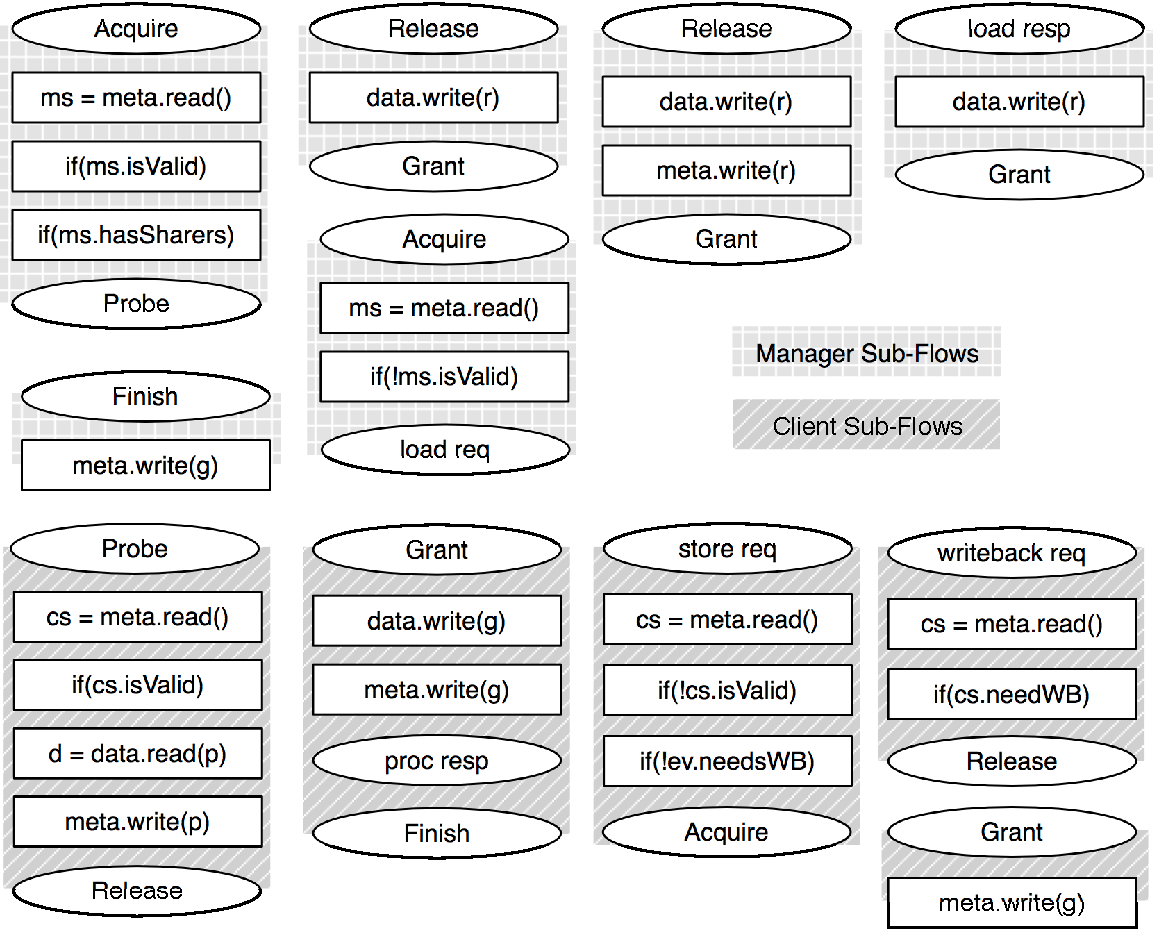
\includegraphics[width=1\columnwidth]{coherence/figures/decoupled.pdf}
\caption[Decomposing sub-flows based on location.]{
We can decompose flows into sub-flows, and collect sub-flows that occur within the same agent.
}
\label{fig:decomp-flow}
\end{figure}

Once we have partitioned all the global flow DAGs into smaller DAGs representing local sub-flows,
it is trivial to collect the set of sub-flows that correspond with a particular agent type.
Figure~\ref{fig:decomp-flow} illustrates an example decomposition using the three flows from the previous section.
Each sub-flow begins and ends with some kind of messaging event.
Note how some of the sub-flows were duplicated across the original flows and have been deduplicated here;
this deduplication is the basis of some significant opportunities for code reuse.

The per-agent-type subset of sub-flows then forms the basis of the operations that we will expect this agent to be able to perform atomically.
In the next section, we discuss how to turn any of these collections of localized sub-flows into a cache or directory controller.

\subsection{Implementing Local Sub-Flows and Their Dependencies}

Given a collection of sub-flows that must be implemented by the particular agent we are designing,
our task is now to implement the control logic that allows those sub-flows to operate atomically.
Ideally, we would be able to perform this transformation automatically, 
but for now some hand-coding is still required in our Rocket Chip Genereatorr~\cite{rocket}.
However, we are able to use Scala to create very concise descriptions of sub-flow behaviors,
which are easily composed together to create complete cache controllers.

Part of our strategy is to create \emph{Transaction Status Handling Registers} (TSHRs).
These modules contain all the state needed to track the progress of 
one type of sub-flow with some handlers capable of merging multiple sub-flows.
We provide a way to execute the actions themselves, as well as to implement the dependencies between actions for each flow.
Actions include reading and writing the metadata and data arrays,
performing atomic memory operations (AMOs),
as well as sending TileLink messages and waiting for matching responses.

We want to factor our HDL code such that code describing common sub-flow actions and their relative ordering dependencies
are well encapsulated, but still made available to each TSHR that uses them as part of its particular sub-flows.
Scala's traits and mix-in multiple inheiritance are a ideal match for this source code factoring task,
as we will show in the following examples.
Each trait consists of functions that actually update state or send a message,
and bits that are added to a ``scoreboard''~\ref{thornton1964scoreboard} that tracks the progress of concurrent sub-flows.
As execution of the sub-flow progresses, additional actions are performed once their dependencies are satisfied.

Dependencies among sub-flows from different traits are expressed inside of the TSHRs themselves,
by referencing the pending bits and providing an additional layer of inter-flow dependencies.
Trackers also contain code to implement the global rules restricting what flows are allowed to execute at the same time.
This step is the portion of the system that we could,
but do not yet, derive automatically from the global flows.
However, we have found that expressing the dependencies via sub-flow pending bits is conscise and much easier to reason about than
constructing interacting state machines to handle each sub-flow. 

\begin{figure}
\centering
\begin{scala}
trait AcceptsVoluntaryReleases extends HasVoluntaryReleaseMetadataBuffer {
  lazy val pending_irel_data = Reg(init=Bits(0, width = innerDataBeats))
  lazy val pending_vol_ignt = connectTwoWayBeatCounter(up = io.inner.release, down = io.inner.grant)

  def irel_can_merge: Bool
  def irel_same_xact: Bool
  def irel_is_accepted: Bool = io.inner.release.fire() &&
                                 (io.alloc.irel || irel_can_merge || irel_same_xact)
  def irel_is_allocating: Bool = state === s_idle && io.inner.release.valid && io.alloc.irel

  def innerRelease(block_vol_ignt: Bool = Bool(false), next: UInt = s_busy) {
    pending_irel_data := (pending_irel_data & dropPendingBitWhenBeatHasData(io.inner.release))
    
    when(irel_is_allocating) {
      xact_addr_block := io.irel().addr_block
      state := next
    }
    
    when(io.inner.release.fire()) {
      when(io.alloc.irel || (irel_can_merge && io.irel().first())) {
        xact_vol_irel := io.irel()
        pending_irel_data := Mux(io.irel().hasMultibeatData(),
                                dropPendingBitWhenBeatHasData(io.inner.release),
                                UInt(0))
      }
    }
    
    io.inner.grant.valid := (state === s_busy || state === s_inner_probe) &&
                              pending_vol_ignt &&
                              !(pending_irel_data.orR || block_vol_ignt)
    
    io.inner.grant.bits := inner_coh.makeGrant(xact_vol_irel)
    
    scoreboard += (pending_irel_data.orR, pending_vol_ignt)
  }
}

\end{scala} 
\caption[The AcceptsVoluntaryReleases trait.]{
The \code{AcceptsVoluntaryReleases} trait contains the \code{innerRelease} function that generates the logic associated with this sub-flow,
which accepts Releases from clients and issues acknowledging Grants.
}
\label{fig:volreltrait}
\end{figure}

\begin{figure}
\centering
\begin{scala}
trait EmitsInnerProbes extends HasBlockAddressBuffer
    with HasXactTrackerStates
    with HasPendingBitHelpers {
  def io: HierarchicalXactTrackerIO

  val pending_iprbs = Reg(UInt(width = innerNCachingClients))
  val curr_probe_dst = PriorityEncoder(pending_iprbs)

  lazy val pending_irels = connectTwoWayBeatCounter(up = io.inner.probe, down = io.inner.release)

  def full_representation: UInt
  def initializeProbes() { pending_iprbs := full_representation & ~io.incoherent.toBits }
  def irel_same_xact = io.irel().conflicts(xact_addr_block) &&
                         !io.irel().isVoluntary() &&
                         state === s_inner_probe
                         
  def innerProbe(prb: Probe, next: UInt) {
    pending_iprbs := pending_iprbs & dropPendingBitAtDest(io.inner.probe)
    io.inner.probe.valid := state === s_inner_probe && pending_iprbs.orR
    io.inner.probe.bits := prb

    when(state === s_inner_probe && !(pending_iprbs.orR || pending_irels)) {
      state := next
    } 
    
     scoreboard += (pending_iprbs.orR, pending_irels)
  } 
} 

\end{scala} 
\caption[The EmitsInnerProbes trait.]{
The \code{EmitsInnerProbes} trait defines the \code{innerProbe} method that generates the logic associated with this sub-flow,
which sends Probes to clients and awaits acknowledging Releases.
}
\label{fig:probetrait}
\end{figure}

We now show examples of some examples of traits containing methods that generate logic implementing sub-flow actions.
Figure~\ref{fig:volreltrait} shows the \code{AcceptsVoluntaryReleases} trait, which accepts voluntary writebacks from clients,
writes the data to some kind of backing storage (which may be local or require further messaging),
and then acknowledges the writeback with a Grant message to the original client.
Note that this trait provides an output hook for ensuring that the intial Release is completed
and an input hook for ensuring that the writeback has been committed to some kind of backing memory.
Figure~\ref{fig:probetrait} shows the \code{EmitsInnerProbes} trait, which send Probes to clients in order to prompt them to Release permissions on a cache block.
The tracker must wait until an appropriate number of Release acknowledgements or writebacks have been collected before advancing
to the next stage, and this trait provides an output hook to do so.
The two traits are composable, in that a particular tracker generator can mix-in both so as to handle Release associated with
both voluntary writebacks and probe responses.

\begin{figure}
\centering
\begin{scala}
class CacheVoluntaryReleaseTracker(trackerId: Int)(implicit p: Parameters)
    extends VoluntaryReleaseTracker(trackerId)(p)
    with HasDataBuffer
    with WritesToOuterCacheDataArray {
  val io = new L2XactTrackerIO

  // Avoid metatdata races with writebacks
  routeInParent(iacqMatches = inSameSet(_, xact_addr_block))

  // Initialize and accept pending Release beats
  innerRelease(
    block_vol_ignt = pending_writes.orR,
    next = s_meta_read)

  io.inner.release.ready := state === s_idle || irel_can_merge || irel_same_xact

  // Begin a transaction by getting the current block metadata
  metaRead(io.meta, s_busy)

  // Write the voluntarily written back data to this cache
  writeDataArray(add_pending_bit = addPendingBitWhenBeatHasData(io.inner.release))

  // Wait for any pending sub-flows
  quiesce(s_meta_write)

  // End a transaction by updating the block metadata
  val new_meta = 
    L2Metadata(
      tag = xact_addr_tag,
      inner = xact_old_meta.coh.inner.onRelease(xact_vol_irel),
      outer = Mux(xact_vol_irel.hasData(),
                  xact_old_meta.coh.outer.onHit(M_XWR),
                  xact_old_meta.coh.outer)),
  metaWrite(io.meta, new_meta, s_idle)       
}
\end{scala} 
\caption[The CacheVoluntaryReleaseTracker.]{
The CacheVoluntaryReleaseTracker is intialized upon receiving a voluntary writeback Release.
It reads the current state of the block from the metadata array, writes backs the new dirty data,
and updates the metadata array.
}
\label{fig:volreltracker}
\end{figure}

\begin{figure}
\centering
\begin{scala}

\end{scala} 
\caption[The BroadcastAcquireTracker.]{
The BroadcastAcquireTracker.
}
\label{fig:acqtracker}
\end{figure}

Trackers are composed of these traits, and additionally consist of logic to manage dependencies among the sub-flows.
They do this by referencing names bits in the scoreboard logic.
Figure~\ref{fig:volreltracker} outlines \code{CacheVoluntaryReleaseTracker}, a tracker that combines the
\code{WritesToOuterCacheDataArray}, \code{AcceptsVoluntaryReleases}, and \code{HasDataBuffer} traits.
This tracker guarantees forward progress in a hierarchical cache by always being available to sink voluntary writebacks.
Figure~\ref{fig:acqtracker} summarizes \code{BroadcastAcquireTracker}, a tracker that combines the
\code{BroadcastsToAllClients}, \code{AcceptsVoluntaryReleases}, 
\code{EmitsVoluntaryReleases}, \code{AcceptsInnerAcquires}, \code{EmitsInnerProbes}, \code{EmitsOuterAcquires},
and \code{HasDataBuffer} traits.
This tracker is used in conjuction with in a broadcast-based messaging medium to handle Acquire transactions
and is an example of combining two traits that use the same messaging channel.

These traits and TSHRs, which are derived from common sub-flows and from global flows respectively,
demonstrate how we are able to transform high-level descriptions of protocol behavior into HDL descriptions
that produce synthesizeable hardware.
The scoreboard logic they produce and compose manages concurrency and atomicity within the agent.
However, we have not yet discussed how policy-specific decisions are expressed within the flows,
and how we can abstract such decisions such that the same tracker designs can be used for multiple protocols.
This policy-centric abstraction is the focus of the next section.

\section{Object-Oriented Coherence Policies}

As in the previous chapter, we distinguish between coherence policies and coherence protocols.
A coherence {\em policy} governs how the Single-Writer-Multiple-Reader invariant is represented as metadata identifying available permissions on data blocks.
A coherence {\em protocol} specifies the exact flows of messages and actions that must be propagated through the memory hierarchy in order to effect a policy.
While decomposing flows into sub-flow traits has proven to be an effective strategy for managing concurrency and complexity in cache controller design,
this approach does not address how different coherence policies are represented within the flows.
For example, what do the state update functions actually store in the metadata arrays?
How are the specific messages required to be sent between agents actually created?
These questions are a matter of policy.

In this section, we present an interface that allows protocol designers to answer these questions
in a well-factored way.
Our goal in introducing this abstract interface is to hold some parts of the controller design constant,
swapping out only the elements of controllers that differ across different policies.
To this end, we have created a unified \emph{CoherencePolicy} interface
that provides the functionality required to fill out the implementation of
all required sub-flows generated by our global flow decomposition.
Specifically, we propose an object-oriented API that is
based around an abstraction of coherence policy metadata.

\emph{Metadata objects} are the fundamental abstraction used in this interface.
These objects are opaque sets of bits which are evaluated and mutated by the coherence policy.
In the object-oriented programming (OOP) paradigm, ``objects'' are abstractions that contain \emph{fields} of data that are mutated and accessed by procedural \emph{methods}.
In OOP, computer programs are designed by making them out of objects that interact with one another.
In our case, we are forming critical portions of the cache controller logic by interacting with objects representing
the metadata about cache block permissions that is stored in local memories.

One advantage of deploying this particular abstraction is that
the specific format and contents of the metadata can be changed without changing the methods that cache controller transactions
use to generate control logic.
This encapsulation allows these aspects of the cache controller to be developed independently
and different metadata implementations and policies to be easily swapped for one another.
By making calls to the methods of these metadata objects, cache controller designers can
create state machines or sub-flow transactions
that cleanly and correctly implement metadata updates. 
Conversely, designers of new coherence protocols are provided a framework
within which to implement their desired policy;
by filling out the response to each method call, they can be certain that the policy
will be applied correctly across any compatible cache or directory controller.

Recall from the previous chapter that TileLink supports hierarchical nesting of protocols via the Manager-Client Pairing (MCP) framework~\cite{beu2011manager}.
Based on this hierarchical structure, we are required to define two distinct types of Metadata objects,
one for agents that act as clients and one for agents that act as managers.
\emph{ClientMetadata} store the permissions available to a client as it attempts to 
apply incoming memory operations to a particular block of cached data.
They may also store protocol-specific information about the block, such as whether or not it has been dirtied by a write.
\emph{ManagerMetadata} store information about how the block has propagated through the clients for which this manager is responsible.
This information might include some representation of the number of client sharers, or patterns of movement observed on that block.
Any agent with access to a particular type of metadata is capable of utilizing the methods
available on that metadata inside of its sub-flow transactions,
and particular agents can store and utilize either or both types.
For example, L1 caches store only ClientMetada, directories or last-level caches store only ManagerMetadata,
caches that are intermediate in the hierarchy may store both types.

The following subsections delineate the specific methods that we provide on each type of metadata.
The methods fall into four main categories.
Permissions check methods compare an incoming operation against the permissions available in the current metadata state,
and they determine whether the operation is allowed to proceed or what kind of followup action to take.
Message creation methods are used to fill in the fields of TileLink message bundles, based on information about the ongoing transaction
and messages that have been received in the past.
Update methods mutate the metadata in response to an incoming operation or message.
We also provide functions to fill in metadata values on hardware reset.
Finally, we have defined a further object-oriented extension to the interface, which abstracts ``directory'' information about how copies of
a cache block have been propagated among a manager's clients.

\subsection{Client Metadata} 

A ClientMetadata object consists of a set of bits that represent the ``state'' of a certain cache block,
i.e., the permissions that the policy has made available on that block inside this particular client cache controller.
The metadata may also store other information about the cache block,
for example, whether it has been dirtied by a store operation.
There are three types of method calls that a cache controller can make against ClientMetadata objects:
permissions checks, message creation, and metadata updates.
Permissions are expressed with respect to memory operations, which we define in Appendix~\ref{a.memopcodes}.
When a permissions check fails, the ClientMetadata methods provide the controller logic with information about what actions are required next.
Some of these actions may involve sending TileLink messages to the client's manager, and we provide methods to create those messages
based on the current metadata.
Another action may be to update the local metadata based on the memory operation.
The complete API for ClientMetadata can be found in the Rocket Chip Generator~\cite{rocket} documentation, but we provide a summary here.

\subsubsection{Permissions Checks}

These boolean functions answer questions about the permissions on a cache line, and in particular,
are used to determine what actions to take relative to specific memory operations.
Memory operation representations are discussed in Appendix~\ref{a.memopcodes}, but the salient feature is that
all of them require either read or read-and-write permissions.

\begin{description}
\item[isValid():]
Is the block's data present in this cache?
\item[isHit(opcode: UInt):]
Does this cache have permissions on this block sufficient to perform the specified memory operation?
If true, the controller can perform the memory operation immediately.
\item[isMiss(opcode: UInt):]
Does this cache lack permissions on this block sufficient to perform the specified memory op?
If true, the controller needs to initiate a TileLink coherence transaction using \code{makeAcquire}.
\item[requiresAcquireOnSecondaryMiss(first: UInt, second: UInt):]
Does a secondary miss on the block require another Acquire message?
If true, in a controller that supports miss-under-miss transactions, initiate a second coherence transaction using \code{makeAcquire}.
\item[requiresReleaseOnCacheControl(opcode: UInt):]
Does a cache control operation (e.g., a voluntary flush) require a Release message to be sent to outer memory?
If true, the controller needs to initiate a TileLink coherence transaction using \code{makeVoluntaryRelease}.
\item[requiresVoluntaryWriteback():]
Does an eviction caused by a capacity miss require a Release to be sent to outer memory?
If true, the controller needs to initiate a TileLink coherence transaction using \code{makeVoluntaryWriteback}.
\end{description}


\subsubsection{Message Creation}

These functions return TileLink channel bundles,
which are constructed  based on a combination of the current metadata state
and particular memory operation types.

\begin{description}
\item[makeAcquire(opcode: UInt, id: UInt, addr: UInt):]
Constructs an Acquire message, based on this metadata, for a memory operation.
\item[makeVoluntaryRelease(opcode: UInt, id: UInt, addr: UInt, data: UInt):]
Constructs a Release message, based on this metadata, for a cache control op.
\item[makeVoluntaryWriteback(id: UInt, addr: UInt, data: UInt):]
Constructs a Release message, based on this metadata, for a capacity eviction.
\item[makeRelease(prb: Probe, data: UInt):]
Constructs a Release message, based on this metadata, in order to respond to a Probe message from outer memory.
\end{description}

\subsubsection{Metadata Updates}

These functions return mutated ClientMetadata objects whose internal state has been updated
based on a particular coherence event or received message type.

\begin{description}
\item[onHit(opcode: UInt):]
New metadata after an operation hits on this cache block.
\item[onCacheControl(opcode: UInt):]
New metadata after an operation releases permissions on this block.
\item[onProbe(incoming: Probe):]
New metadata after receiving a Probe message.
\item[onGrant(incoming: Grant, pending: UInt):]
New metadata after receiving a Grant message in response to the pending memory operation.
\item[onReset():]
New metadata initialized after machine reset.
\end{description}

\subsection{ManagerMetadata} 

A ManagerMetadata object consists of a set of bits that represent the ``state''
of a particular cache block,
i.e., the existence of copies of that block in any client caches
managed by this agent.
The metadata may also store other information about the cache block,
for example, information about its history, pattern of movement between clients,
or ``ownership'' by clients.
As with ClientMetadata, there are three types of method calls
that an agent can make against ManagerMetadata objects:
permissions checks, message creation, and metadata updates.
Messages created by managers include Probes of their clients to trigger them
to Release permissions and Grants of additional permissions to clients
trying to Acquire them.
In addition to these method calls, ManagerMetadata incorporates an additional
object-oriented abstraction, DirectoryRepresentation, which encapsulates
how information about the location of copies of the managed cache blocks is stored.
The complete API for ManagerMetadata can be found in the
Rocket Chip Generator documentation~\cite{rocket}, but we provide a summary here.

\subsubsection{Permissions Checks}

These boolean functions answer questions about the permissions on a cache block,
and in particular, are used to determine whether it is necessary to Probe any
clients that currently may have copies of a particular cache block,
with respect to a client's request to Acquire new permissions or a
Release of the block from this agent.

\begin{description}
\item[requiresProbes(acq: Acquire):]
Does this Acquire require Probes to be sent to any other clients with copies?
\item[requiresProbes(opcode: UInt):]
Does this memory operation require Probes to be sent to any clients with copies?
\item[requiresProbesOnVoluntaryWriteback():]
Does an eviction caused by a capacity missed require Probes to be sent to any clients with copies?
\end{description}

\subsubsection{Message Creation}

These functions return TileLink channel bundles to use as responses to Clients,
which are constructed  based on the combination of current metadata state and 
past TileLink messages received.

\begin{description}
\item[makeProbe(dst: UInt, acq: Acquire):]
Construct a Probe message based on this metadata in response to a particular Acquire message.
\item[makeProbe(dst: UInt, opcode: UInt, addr: UInt):]
Construct a Probe message  based on this metadata in response to a particular cache control operation.
\item[makeProbeForVoluntaryWriteback(dst: UInt, addr: UInt):]
Construct a Probe message based on this metadata for a capacity eviction.
\item[makeGrant(rel: Release, id: UInt):]
Construct an appropriate Grant message to acknowledge a Release message.
\item[makeGrant(acq: Acquire, id: UInt, data: UInt):]
Construct an appropriate Grant message to acknowledge an Acquire message.
May contain single or multiple beats of data, or just be a permissions upgrade.
\item[makeGrant(pri: Acquire, sec: SecondaryMissInfo, id: UInt, data: UInt):]
Construct an appropriate Grant message to acknowledge an Acquire message, overriding some fields
Used to respond to secondary misses merged into this transaction.
May contain single or multiple beats of data.
\end{description}

\subsubsection{Metadata Updates}

These functions return mutated ManagerMetadata objects whose internal state has been updated based on a particular coherence event or TileLink message.

\begin{description}
\item[onRelease(incoming: Release):]
New metadata after receiving a Release message.
\item[onGrant(outgoing: Grant):]
New metadata after sending a Grant message.
\item[onReset():]
New metadata initialized after machine reset.
This method can also be used to generate a generic ManagerMetadata object to access other API methods
within controllers that do not store any metadata (for example a bus controller).
\end{description}

\subsubsection{Directory Representation}

As a member of the ManagerMetadata objects,
we also provide an object-oriented API for accessing and maintaining directory information.
These directory objects are responsible for tracking the propagation of cache blocks
across all the clients under the purview of a particular manager.
They abstract the details of the storage format used in the directory portion of the ManagerMetadata.
For example, rather than using a full bit vector (where every bit represents whether or not a particular client contains a copy of the data block),
a designer might instead choose to use a coarser representation
or one based on a limited set of pointers to individual sharers~\cite{sorin2011primer}.
Our goal was to allow the directory representation to be changed independently from
the rest of the cache coherence policy or controller design.
These DirectoryRepresentation objects' methods are intended to be called
from within the CoherencePolicy's ManagerMetadata functions by policy authors,
rather than externally by controller designers.
The methods currently included in the DirectoryRepresentation API are:
\begin{description}
\item[pop(id: UInt):] Remove id from the prior set of sharers, returning a new set.
\item[push(id: UInt):] Add id to the set of sharers, returning a new set.
\item[flush():] Provide an empty set that indicates no sharers.
\item[none():] True if there are no shared copies among clients.
\item[one():] True if there is a single copy at a client.
\item[count():] Total count of the sharers among clients.
\item[next():] Provide the id of the client that should be Probed next.
\item[full():] Provide a full bitmap of all sharers, where a 1 indicates a copy.
\end{description}

Our intention when designing this inteface was to provide a way for CoherencePolicies
to find out all information about sharer propagation that they need to operate correctly,
without having to explicitly refer to the particular bits of the representation
stored in the agents' metadata array.
As we define additional policies and representations,
we may expand this interface to address other questions.

\subsection{Creating New Coherence Policies}

So far we have discussed the object-oriented API that our methodology provides to
protocol flow and cache controller designers, which presents them with coherence metadata objects
to manipulate.
We now discuss provisioning the other side of the interface, from the perspective
of developers of new coherence policies.

We give designers planning to implement new coherence policies several Scala traits
containing abstract declarations of a variety of methods, which are themselves in turn
used to implement the coherence metadata object methods discussed in the previous subsections.
These three traits are combined to form the complete \code{CoherencePolicy} interface.
The three traits are:
\begin{description}
\item[HasCustomTileLinkMessageTypes] defines the custom, coherence-policy-defined message types, as opposed to the built-in ones. Policies must enumerate the custom messages to be sent over each channel, as well as which of them have associated data.
\item[HasClientSideCoherencePolicy] contains all functions required for client coherence agents. Policies must enumerate the number of client states and define their permissions with respect to memory operations. Policies must fill in functions to control which messages are sent and how metadata is updated in response to coherence events.
\item[HasManagerSideCoherencePolicy] contains all functions required for manager coherence agents. Policies must enumerate the number of manager states. Policies must fill in functions to control which Probe and Grant messages are sent and how  metadata should be updated in response to coherence events.
\end{description}

By filling in the missing implementations of the methods defined in these traits, 
coherence policy developers can provide a complete coherence policy
that will interoperate seamlessly with our supplied cache controllers and TileLink networks.
It is possible to reuse implementations of certain traits to improve code reuse across \code{CoherencePolicy} implementations,
in cases where a Client or Manager agent's behavior is the same as under another policy.
In either case, a concrete \code{CoherencePolicy} subclass provides implementations for every method.
An instance of such a class is a Scala object that can be passed through a hierarchy of
Chisel Modules and used by any associated coherence metadata object implementations.
We discuss the parameterization of the memory system components by \code{CoherencePolicies}
in the next section.

The complete API for the \code{CoherencePolicy} interface can be found in the
Rocket Chip Generator documentation~\cite{rocket}.
It is similar enough to the \code{ClientMetadata} and \code{ManagerMetadata} interfaces that
we do not reproduce it here.
The differences mainly revolve around taking the state information encapsulated
in Metadata objects and making them explicit parameters of the CoherencePolicy methods.
Under this organization, the functions defined in these traits
are called from within the \code{ClientMetadata} and \code{ManagerMetadata} member methods.
This encapsulation means that the internals of those classes do not have to be changed
when new coherence policies are defined.
Similarly, if we change the Metadata representations in the future,
modules which use the Metadata objects' methods will not have to be changed.

The decisions captured by the \code{CoherencePolicy} are exposed to cache controller authors through
the coherence metadata objects.
As discussed in more detail in the next section,
an additional advantage of this organization is that the Parameters object
associated with the coherence metdata object can be used to set the widths of the fields of the
TileLink channel bundles that are the outputs of many of the inteface's methods.

\section{Parameterization and Coherence Policies}

In this section we will discuss the interplay between Context-Dependent Environments (CDEs),
which we introduced in Chapter~\ref{c.parameters},
and the CoherencePolicy and Metadata objects.
CoherencePolicy objects are parameterized by the DirectoryRepresentation that they use.
More complicated policies could potentially be additionally parameterized in order to tune their heuristic behavior.
Metadata objects are parameterized by the TileLinkParameters objects of the TileLink network with which they are associated.
Figure~\ref{fig:cdepolicy} illustrates these relationships.

\begin{figure}[t!]
\centering
%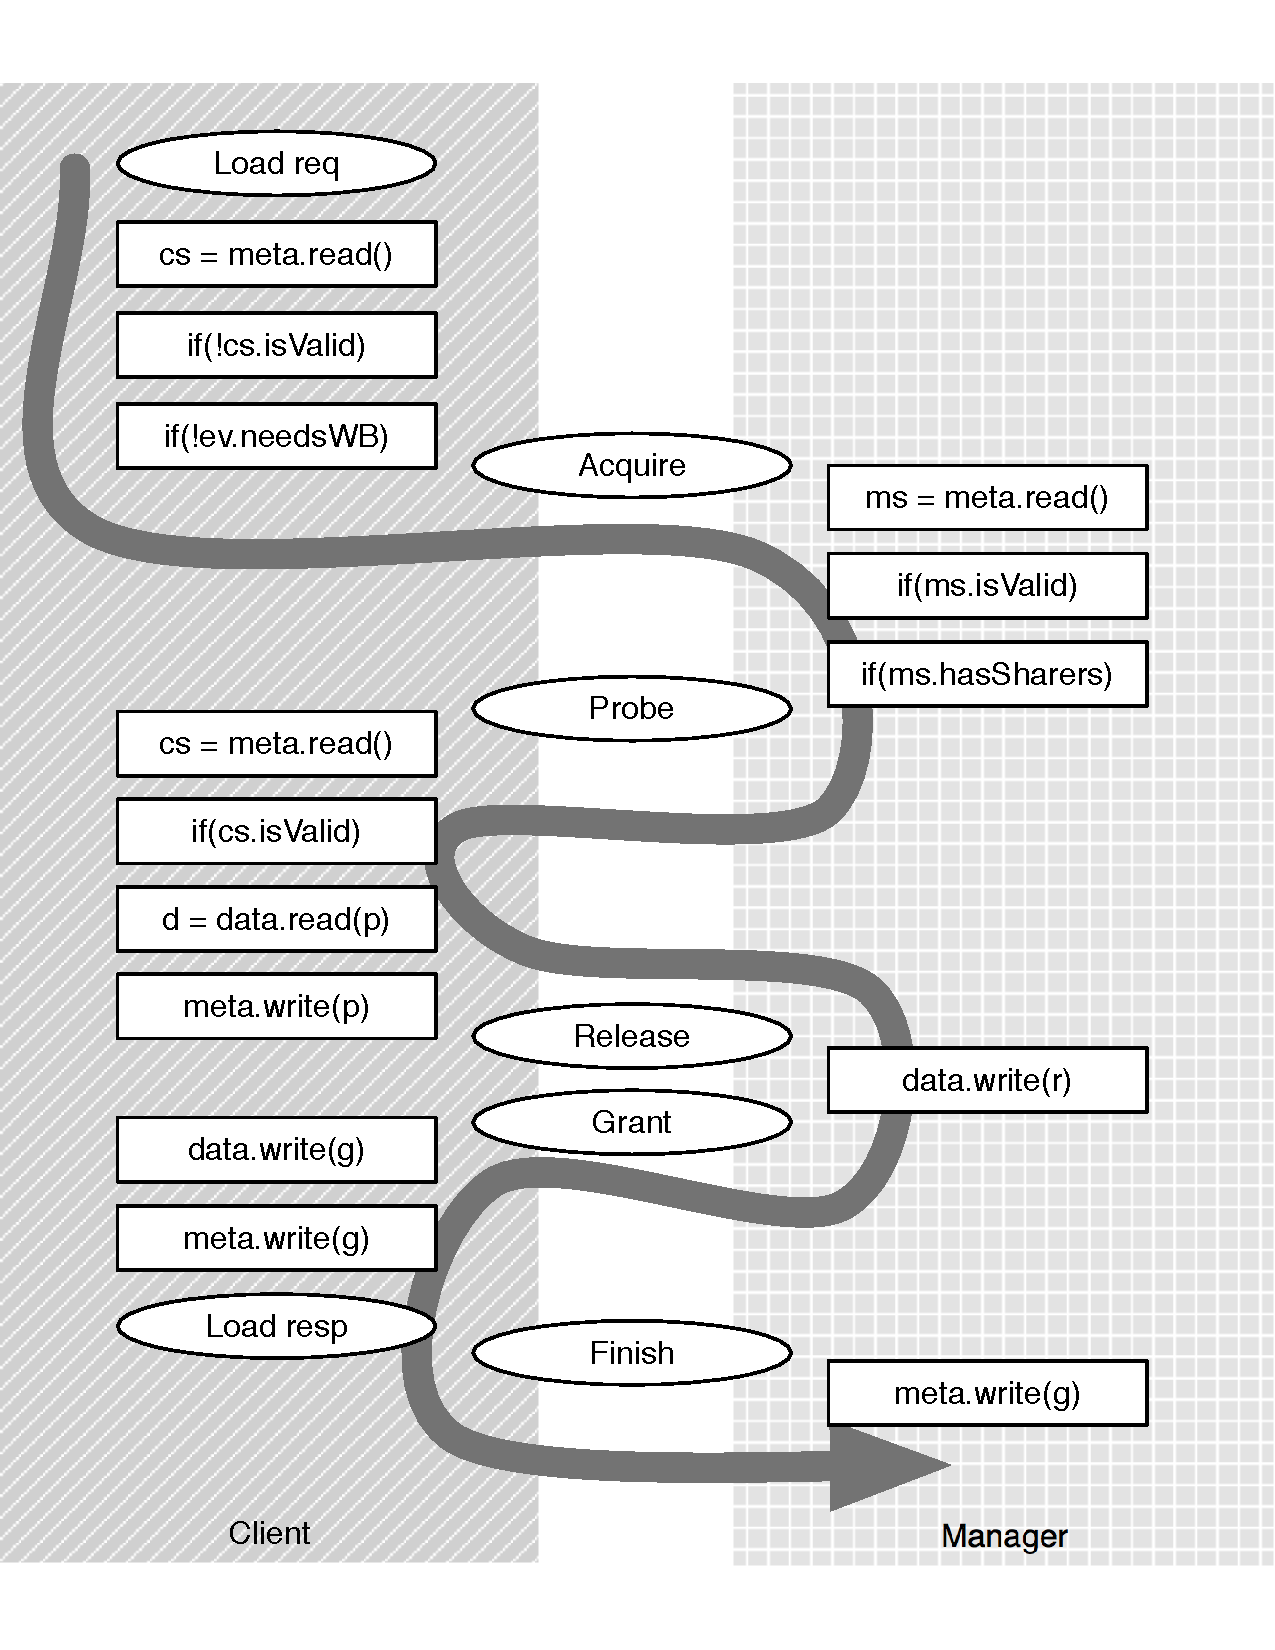
\includegraphics[width=1\columnwidth]{coherence/figures/cdepolicy.pdf}
\caption[Parameterizing Coherence Policies.]{
Parameterizing Coherence Policies.
}
\label{fig:cdepolicy}
\end{figure}

We include a CoherencePolicy as a member of the TileLinkParameter case class that stores all the information
about channel widths associated with a particular TileLink realm (see Chapter~\ref{s.tlparam}).
In other words, there is a one-to-one mapping between CoherencePolicies and TileLink networks.
However, we can use the context-dependent capability of our CDEs to 
inject multiple TileLink realms into a single controller,
which allows us in turn to stitch together multi-level protocols through hierarchical agents
that have coherence metadata objects associated with each TileLink realm.

TileLinkParameters are therefore associated with and used by the coherence policy metadata objects.
Specifically, the ``geographical'' parameter \code{TLKey} is set based on whether the metadata belongs to the inner or outer realm.
Thus, in hierarchical agents with multiple types of metadata objects, accessing the methods
discussed in this chapter automatically and correctly parameterizes the width of the bundles those methods produce.
This organization reduces code complexity by automatically determining the correct set of TileLinkParameters to use to produce data on a particular channel,
as well as to reference the correct coherence policy when making flow control decisions in a hierarchical system.

\section{Hierarchical Translation Between Protocols}

TileLink supports a hierarchical transaction structure that allows protocol transactions
to be nested inside one another, as we discussed in Chapter~\ref{s.tlhier}
based on the MCP framework proposed by \cite{beu2011manager}.
Building off of this capability, our goal is to enable different coherence policies to be employed at each level,
depending on that level's particular scale and requirements.
At the protocol level, this means that when sub-flows of a protocol transaction
occur in different coherence realms, we need to provide capabilities for
new sub-flows to be initiated based on information taken from the previous sub-flow
that happened in the other realm.
Doing so requires a translation between inner and outer realms,
which we facilitate via memory operation codes and the
coherence metadata object methods previously discussed in this chapter.

A set of pre-defined memory opcodes
form an interface through which different policies in our protocol family can communicate.
Appendix~\ref{a.memopcodes} delineates the current set of opcodes used in the Rocket Chip generator.
The salient detail is that these operations encode information about whether read permission or write permission
must be acquired or released in order to effect the desired operation.

Any hierarchical agent has both ClientMetadata (associated with the outer realm)
and ManagerMetadata (associated with the inner realm).
Performing a translation between realms necessitates utilizing methods on both types of metadata objects,
based on the TileLink messages that triggered the new inner or outer sub-flow.
TileLink determines the ordering/interleaving of the outer transaction with the inner transaction;
and the CoherencePolicy's job is to determine which translated transaction is needed.
There are two pairs of TileLink messages that cross realm boundaries,
Acquire/Grant and Probe/Release.
We discuss each in turn.

To continue an Acquire transaction originating in the inner realm
by initiating a sub-flow in the outer coherence realm, we check the opcode
of the original transaction's Acquire message against the ClientMetadata stored in this agent.
If the metadata indicates that an outer transaction is required, this agent (acting as a client),
sends a further request to its manager and awaits a Grant response.

Another translation occurs when a hierarchical agent receives a Probe message from
the outer coherence realm.
In this case, the outer Probe's opcode must be compared against the permissions stored in the ClientMetadata.
If these permissions would be reduced, the inner realm's ManagerMetadata must be consulted in order
to determine what Probe messages to forward to which agents.
Only after the inner realm's Release messages have been collected can an outer Release message be generated
based on the ClientMetadata.

Overall, TileLink determines the ordering/interleaving of the outer transaction with the inner transaction;
and the CoherencePolicy's job is to determine which outer transaction is needed.
By defining a set of operations in terms of which permissions they acquire or release,
we enable multiple policies to intermesh in the formation of a single, multi-level, hierarchical protocol.


\section{Concrete Protocols in the Rocket Chip Generator}

We now present a family of five protocols that we have implemented using Chisel, TileLink, CoherencePolicy
and our flow-based cache controllers in the Rocket Chip Generator~\cite{rocket}.
These protocols are based around a subset of the classic five state MOESI model
first introduced by Sweazey and Smith~\cite{sweazey1986class}.
The protocols contain some subset of the following stable client metadata states~\cite{sorin2011primer}:
\begin{description}
\item[I:] The block is invalid. The cache either does not contain the block or it contains a potentially stale copy that it may not read or write.
\item[M:] The block is valid, exclusive, owned, and potentially dirty. The block may be
read or written. The cache has the only valid copy of the block, the cache must respond to
requests for the block, and the copy of the block at the LLC/memory is potentially stale. 
\item[S:] The block is valid but not exclusive, not dirty, and not owned. The cache has a read-only copy of the block. Other caches may have valid, read-only copies of the block.
\item[E:] The block is valid, exclusive, and clean. The cache has a read-only copy of the
block. No other caches have a valid copy of the block, and the copy of the block in the
LLC/memory is up to date. 
\end{description}

We have also implemented a more advanced \emph{migratory} protocol. 
This protocol is a reactive protocol, based on proposals by~\cite{stenstrom-isca93,cox-isca93},
that tracks the behavior of cache blocks over time,
identifies migratory behaviors of individual cache blocks,
and proactively Releases permissions on a newly written block in order to make it available to be consumed
with requiring a Probe/Release sub-flow.
The specialization of the protocol to adapt to migratory movement patterns is captured dynamically
by additional Client states.

Table~\ref{tab:protocols} lays out the relative capabilities of these five policies.
The client states that effectively differentiate the protocols are not strictly supersets of one another,
allowing us to choose a protocol appropriate to the context in which it is deployed.

\begin{table}[t] 
\begin{center}
\begin{tabular}{|l|c|c|c|c|c|} 
\hline
Name & C. States & R+W       & RO        & Clean     & Adaptive \\ \hline
MI        & 2 & \ding{52} &           &           & \\ \hline
MEI       & 3 & \ding{52} &           & \ding{52} & \\ \hline
MSI       & 3 & \ding{52} & \ding{52} &           & \\ \hline
MESI      & 4 & \ding{52} & \ding{52} & \ding{52} & \\ \hline
Migratory & 7 & \ding{52} & \ding{52} & \ding{52} & \ding{52} \\ \hline
\end{tabular}
\caption{Overview of features of protocols currently available in the Rocket Chip Generator.}
\label{tab:protocols}
\end{center}
\end{table}

In addition to the five different policies, we also provide three different hierarchical agent implementations.
These include two types of Broadcast networks, and an LXCache.
The LXCache can be used to implement any outer cache.
All the controller implementations can be combined with any policy,
as well as a TileLink-compatible Network-on-Chip (NoC),
in order to make a complete protocol fabric.

The interoperability and abstracts deployed in our memory hierarchy generator allow
the XX lines of Chisel code we use to express the local transactions 
to be reused across the three manager agent implementations.
At the same time,
the YY lines of code used to express each policy share ZZ lines of common policy decision-making logic.
Overall the entire memory generator, including cache storage arrays, networks and converters,
is expressed in less than AA lines of Chisel code.

%Performance measurements, holding design parameters constant (other than core count?).
%Figure~\ref{} shows MI vs MEI for read-only data.
%Figure~\ref{} shows MI/MEI vs MSI/MESI for shared data.
%Figure~\ref{} shows MESI vs Migratory for migratory data.

\section{Discussion}

``The essence of abstractions is preserving information that is relevant in a given context, and forgetting information that is irrelevant in that context''~\cite{guttag2014introduction}.
This chapter has introduced a set of abstractions and interfaces that make it more productive to write extensible coherence protocols.
In that spirit, in this section I attempt to distill the relationships between our various protocol abstractions and highlight which information they encapsulate and expose.


In our paradigm, a protocol consists of many transactional message flows.
Flows may share common sub-flows, which can be codified as local transactions on state
and then mixed together to form controller logic,
with dependencies among sub-flows being inferred from the global flows.
Flows utilize our metadata objects to define policy-based permissions
and and are shaped by our TileLink substrate for deadlock-free ordering.
Figure~\ref{fig:overview} highlights the interplay between message flows, coherence metadata objects, and TileLink.

\begin{figure}[t!]
\centering
%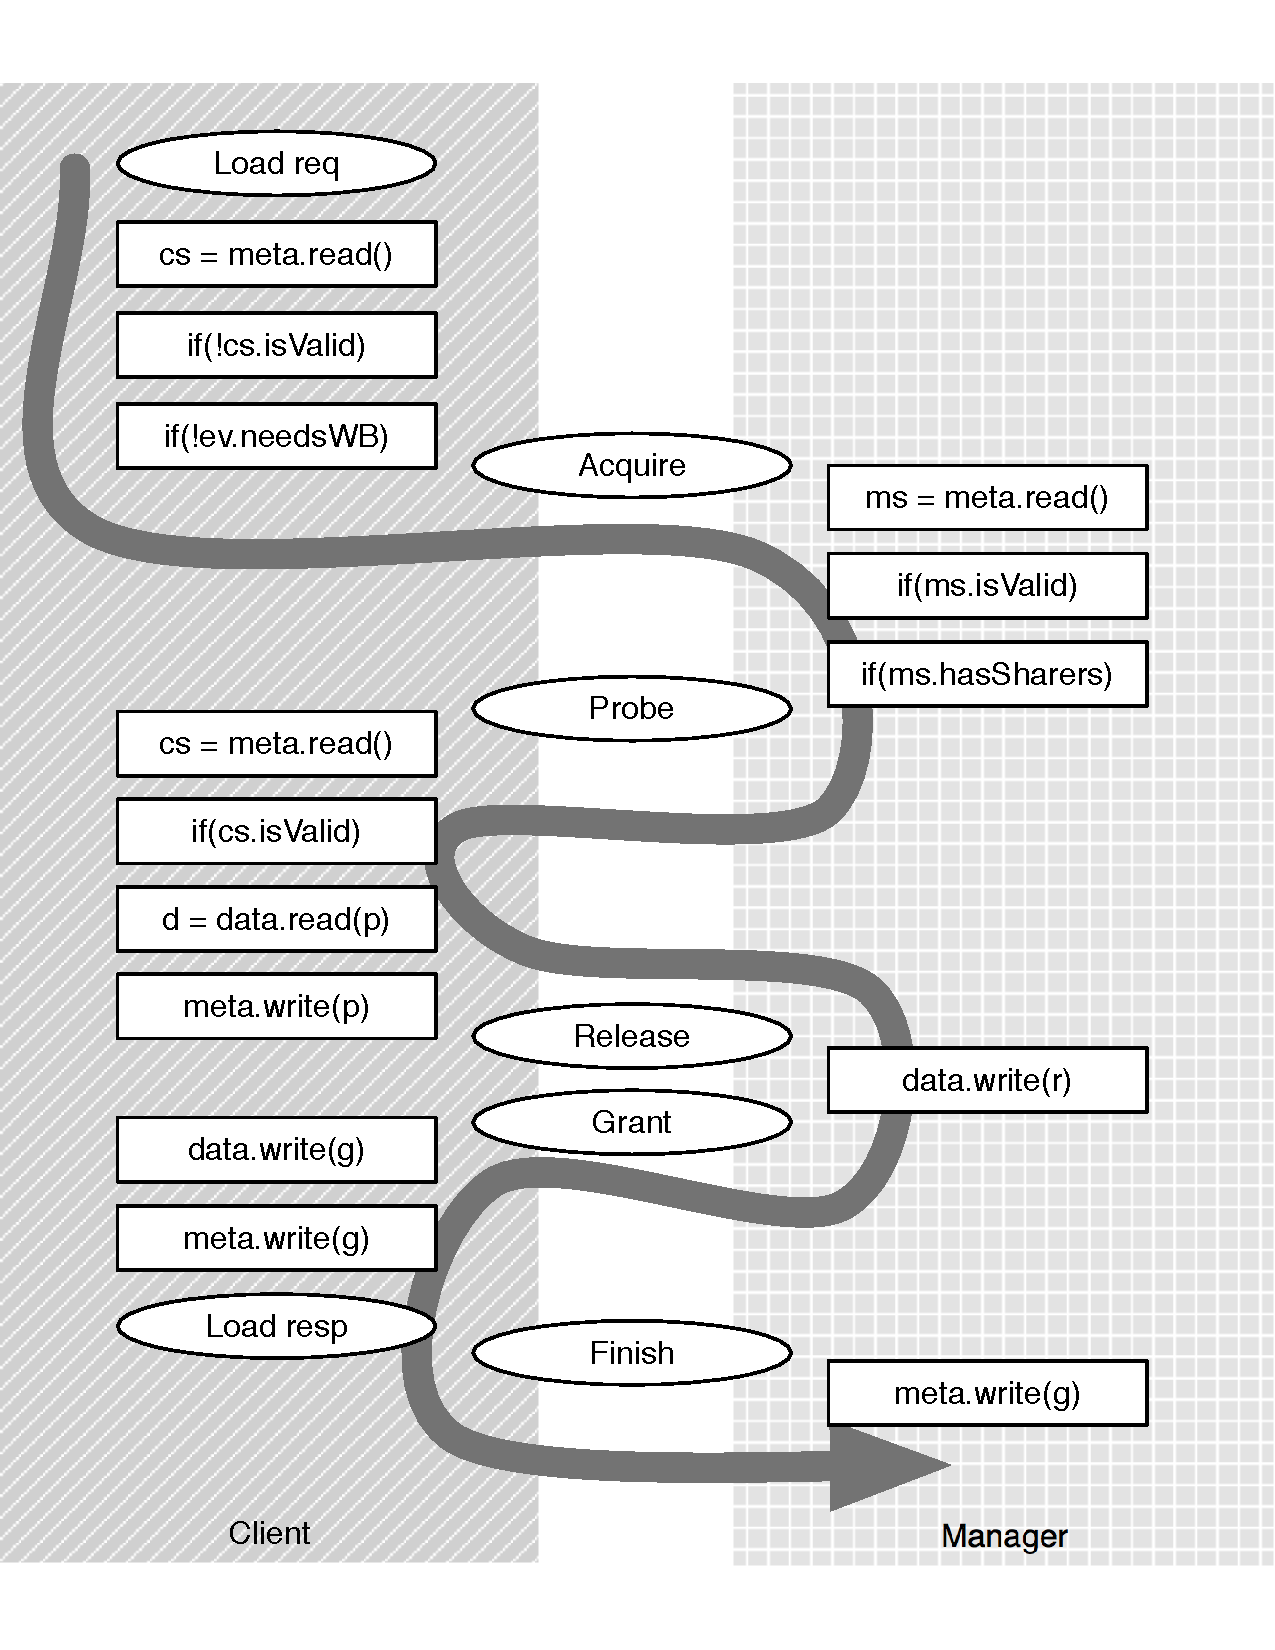
\includegraphics[width=1\columnwidth]{coherence/figures/overview.pdf}
\caption[Separation of Concerns.]{
The separation of concerns between message flows, coherence metadata objects, and the TileLink framework.
}
\label{fig:overview}
\end{figure}

Coherence metadata objects abstract the policy decisions inherent to the protocol.
Queries made against coherence metadata objects act to determine which flow or sub-flow is occuring.
The policy encapsulated by the metadata objects defines the complete set of custom TileLink message types
associated with a particular protocol and determines which ones are sent within a given flow.
A metadata-based policy is not concerned with anything having to do with time or ordering,
only with what action needs to be taken when the system is in a particular state.
This factoring allows multiple policies to be plugged in without changing controller design
or network implementation.

The TileLink framework acts a substrate that guarantees message flows will make forward progress
as long as certain guarantees about agent behavior are satisfied.
The framework thereby determines the possible shapes and relative priorities of flows,
defining several sub-flow shapes that are safe to compose hierarchically.
The framework determines what types of messages any coherence policy methods can possibly output.
It is not concerned with which messages should be sent under what conditions,
just the relative priority and allowed orderings of the general message types.
This factoring allows multiple network implementations to be plugged in without changing controller design
or policy contents.

Message flows act as the glue between the policy control logic and
the network substrate by informing the design of the agent controller logic itself.
In specifying the local sub-flows that occur within each controller type, message flows determine
which policy methods a particular agent calls upon receipt of particular TileLink message types,
how it sends particular message types in response,
and the ordering constraints in data and metadata reads and writes.
This factoring allows the implementation of the cache controller logic
to be changed without requiring changes to the policy description or network implementation.

Taken together, we can see how the trade-offs in information available within each abstraction
help to make protocol design more productive and tractable.
By separating information about timing from policy decisions, policy designers only have to consider
current state and desired operation, yet know what general type of message need be produced.
By eliding information about policy from the networking substrate, NoC designers know what priority channels to provision, without focusing on the details of any one policy.
Agent control logic implementations use both abstractions to simplify their code density and increase code reuse, and
both abstractions provide structure to the high-level, global message flows that can be productively verified.

\section{Future Work}

The most concrete direction for future work in this area is to use our CoherencePolicy interface
in the design of custom protocols that feature additional adaptability features.
These features could involve automatically detecting memory access patterns in hardware
and proactively managing data placement policies accordingly, similar to 
the Migratory policy whose features we discussed in a previous section of this chapter.
Alternatively, we might want to enable hooks to allow for software control of coherence states,
possibly via further memory opcodes targeting individual cache blocks and triggering new transaction flows.
This approach could also involve integration with other software-based data placement strategies, such as VLS~\cite{Cook:EECS-2009-131}.
Appendix~\ref{a.swmem} provides an overview of related work in this area.

Past designs for adaptively coherent shared memory systems, such as Standford FLASH \cite{kuskin-archnews94}, 
have incorporated multiple protocols on top of a single hardware substrate. 
We expect that it will be relatively straightforward  to emulate this strategy by
running multiple protocols on a single TileLink interconnection substrate.
The open question is how best to enable software control over which protocol to use for which data.
For example, should this specialization be specified via a global mode switch, or instead
differentiated for particular memory regions.
The latter implies that multiple protocols would be in operation on the same network at the same time.
Ideally, we will be able to capture such complicated meta-protocols using the same set of interfaces we have defined here.

Moving from investigations of concrete policy designs to the process of designing policies,
we hope that future work will exploit improvements in Chisel functionality to close the remaining gap in
automating the process of producing verification and synthesis from the same description.
While we expect the message flows described in this chapter are compatible with CMP-based tools,
actually automating such a fully integrated verification workflow is not within the scope of this thesis.

The next step in accomplishing the aforementioned verification goal is to furnish capabilities for
automatic generation of controllers via Bluespec-style rules built on top of Chisel.
While this thesis has provided an algorithm for  breaking a set of
global message flow transactions into sets of localized rules,
we still manually implemented the non-interference control logic for those localized rules.
While our current Chisel description is concise enough that is it easier to reason about than the traditional Verilog approach,
it still introduces opportunity for human error in translating the sub-flows and constructing the TSHRs.
A superior approach might be for a Bluespec-style ``rule engine'' generator to automatically infer the control dependencies between sub-flows.
Ideally, future investigations will address the verification advantages of automatically generated rule engines while
contrasting them with the resource efficiency of the hand-written scoreboard logic that we currently deploy.

Along similar lines of attack, we would also ideally be able to automatically infer the implementations of CoherencyPolicy methods
based on a set of decision points extracted from flow descriptions.
For now, the policy methods are filled in manually.
Since we already identify the nodes in the message flow graphs that differentiate the flows by
inroducing divergent sub-flows, it should be possible to re-cast those decision nodes as the implementations of certain methods,
particularly those related to permission checks.

As this toolset matures, we anticipate a wealth of design space exploration opportunities to arise.
The hierarchical nature of TileLink makes it possible to generate arbitrarily nested multi-level memory hierarchies.
Improvements to the Chisel ecosystem are advancing the state of the art in FPGA-based energy consumption modeling.
Future work should deploy these capabilities to measure the efficacy of data movement strategies,
as well as questions related to storage versus communication costs; for example, the coarseness of directory representations.
We hope that our open source frameworks will prove to be a valuable tool for memory hierarchy researchers.

\section{Conclusion}

Cache coherence protocol design is one of the toughest challenges in computer architecture.
Through better abstractions, we have attempted to reduce the burden put on hardware developers
to correctly interpret the implicit semantics of abstract coherence models in their implementations.
We propose a top-down approach to protocol specification based on message flows, and we provide a strategy
for transforming such specifications into Chisel implementations of cache controllers.
We also utilize object-oriented programming to encapsulate the policy-specific decisions encoded
in the flows, making it easy to swap policies without changing any controller HDL source code.
This approach opens the door to more flexible and customizable protocol design, which will be important
to the future of energy-efficiency in the on-chip memory hierarchy.
